\documentclass[../main.tex]{subfiles}

\begin{document}

\subsection{A Test Problem}
In this section we derive and evaluate a number of common numerical schemes for the solution of a test problem: the wave equation in one dimensions
\begin{gather}\label{eq:wave}
    \frac{\partial^2 u}{\partial t^2} = c^2\frac{\partial^2 u}{\partial x^2}\qquad\text{for }(x)\in V,
\end{gather}
where $c$ denotes the propagation speed, and $V$ denotes the interior of our spatial domain. For this equation, we consider homogenous Dirchlet boundary conditions
\begin{gather*}\label{eq:bcs}
    u(t,x) = 0\qquad\text{for }x\in A,
\end{gather*}
where $A$ denotes the exterior of our spatial domain. Finally, we also consider some initial condition
\begin{gather*}\label{eq:ic}
    u(t,x) = f(x)\qquad\text{for }t=t_0.
\end{gather*}
The equation \ref{eq:shallow}  that we plan to numerically solve is very similar to this equation, as both are linear second-order hyperbolic partial differential equations. Further, we will be using the same boundary and initial conditions. Now, given homogeneous Dirchlet boundary conditions and a gaussian initial condition:
\begin{gather*}
    f(x) = e^{-x^2},
\end{gather*}
we know that the exact solution is given by:
\begin{gather*}
    u(t,x) = \frac{1}{2}e^{-(x+ct/2)^2} + \frac{1}{2}e^{-(x-ct/2)^2}.
\end{gather*}
This can be shown using a variety of techniques to solve PDEs, including the Fourier transform. Thus, the initial condition splits into two waves that propagate in opposite directions along the spatial dimension $x$.

\subsubsection{Conservative Form of Test Problem}
\noindent Here, we state our test problem \label{eq:wave} in conservative form. To do this we define variables $\gamma$ and $\alpha$ such that:
\begin{gather*}
    \left.
    \begin{aligned}
        \alpha &= c\frac{\partial u}{\partial x}\\
        \gamma &= \frac{\partial u}{\partial t}
    \end{aligned}
    \right\}
    \Rightarrow
    \mathbf{U} = \begin{bmatrix} \alpha \\ \gamma\end{bmatrix}.
\end{gather*}
Now, we take derivatives with respect to time obtain a coupled system of equations:
\begin{gather*}
    \begin{aligned}
         \frac{\partial \alpha}{\partial t} &= c\frac{\partial^2 u}{\partial t \partial x} = c\frac{\partial^2 u}{\partial x \partial t} = c\frac{\partial \gamma}{\partial x},\\
        \frac{\partial \gamma}{\partial t} &= \frac{\partial^2 u}{\partial t^2} = c \frac{\partial}{\partial x}\left( c \frac{\partial u}{\partial x}\right) = c \frac{\partial \alpha}{\partial x}.
    \end{aligned}
\end{gather*}
We may write this in matrix form by:
\begin{gather*}
\frac{\partial }{\partial t}
\begin{bmatrix}
\alpha\\\gamma
\end{bmatrix}
+
\begin{bmatrix}
\partial_x & 0\\
0 & \partial_x 
\end{bmatrix}
\left(
\begin{bmatrix}
0 & -c\\
-c & 0
\end{bmatrix}
\begin{bmatrix}
\alpha\\\gamma
\end{bmatrix}
\right)
=
\mathbf{0}.
\end{gather*}
Finally, we note that the numerical scheme will need the initial condition $\mathbf{U}(t=0)$. This is obtained by taking $\alpha(t=0)=f'(x)$ and $\gamma(0)=0$.
 
\subsection{The Lax-Wendroff Scheme}
The Lax-Wendroff scheme \cite{rezzolla} is a combination of the Lax-Friedrichs scheme and the leapfrog scheme. Assume that the hyperbolic PDE of interest has been stated in the conservative form:
\begin{gather*}
    \frac{\partial \mathbf{U}}{\partial t} + \nabla \cdot \mathbf{F}(\mathbf{U}) = 0.    
\end{gather*}
The first step is to compute two half-steps, from Lax-Friedrichs:
\begin{gather*}
    \begin{aligned}
	   \mathbf{U}^{n+1/2}_{j+1/2} &= \frac{1}{2}(\mathbf{U}^{n}_{j+1}+\mathbf{U}^{n}_{j}) - \frac{\Delta t}{2\Delta x}(\mathbf{F}^{n}_{j+1}-\mathbf{F}^{n}_{j}),\\
       \mathbf{U}^{n+1/2}_{j-1/2} &= \frac{1}{2}(\mathbf{U}^{n}_{j}+\mathbf{U}^{n}_{j-1}) - \frac{\Delta t}{2\Delta x}(\mathbf{F}^{n}_{j}-\mathbf{F}^{n}_{j-1}).
    \end{aligned}
\end{gather*}
Now, the flux density $\mathbf{F}$ is evaluated at these half-steps:
\begin{gather*}
    \mathbf{F}^{n+1/2}_{j\pm1/2} = \mathbf{F}\left(\mathbf{U}^{n+1/2}_{j\pm1/2}\right).
\end{gather*}
These are then used in the computation of a leapfrog half-step:
\begin{gather*}
	\mathbf{U}^{n+1}_{j} = \mathbf{U}^{n}_{j}-\mathbf{F}\left(\mathbf{U}^{n+1/2}_{j+1/2}-\mathbf{U}^{n+1/2}_{j-1/2}\right).
\end{gather*}
A stencil is given from Rezolla \cite{rezzolla} illustrating this process in figure~\ref{fig:lw}.
\begin{figure}[H]
    \centering
    \fbox{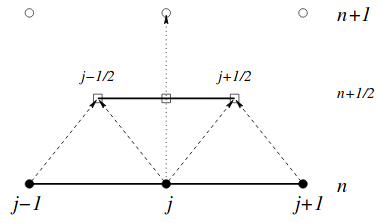
\includegraphics[width=0.75\textwidth]{lw}}
    \caption{Stencil of the Lax-Wendroff Scheme}
    \label{fig:lw}
\end{figure}
\subsection{Stability of Lax-Wendroff}
In order for Lax-Wendroff to be a stable scheme, the time and spatial discretizations must exactly meet the \textit{Courant-Freidrichs-L\"owry condition} \cite{rezzolla}:
\begin{gather*}
    \frac{|v_{\text{max}}|\Delta t}{\Delta x} = 1,
\end{gather*}
where $v_{\text{max}}$ is the maximum velocity of the wave. In practice, this is used to determine the timestep of our method given a spatial discretization:
\begin{gather*}
    \Delta t = \frac{\Delta x}{|v_{\text{max}}|}.
\end{gather*}
This choice ensures that the propagation speed of the wave is always smaller than the numerical speed of the wave $\Delta x / \Delta t$ \cite{rezzolla}.

\subsection{Boundary Conditions}

Our first implementation of Lax-Wendroff applied to the wave equation implemented Dirichlet boundary conditions, with the solution at the endpoints being set to $0$. This caused numerical instability in the solution which worsened as the number of time steps used in the discretization increased. Our solution to this was to implement Sommerfeld boundary conditions (also called radiative boundary conditions). These boundary conditions allow the wave to freely move out of our system when it reaches the boundary by applying a numerical scheme for basic advection \cite{rezzolla}. The following numerical scheme was implemented to allow the waves to advect from the system:

\begin{gather*}
	\mathbf{U}^{n+1}_{j+1} = \mathbf{U}^n_j - \mathbf{U}^{n+1}_jQ+\mathbf{U}^n_{j+1}Q,	
\end{gather*}

\noindent for the outer (positive x) edge and 

\begin{gather*}
	\mathbf{U}^{n+1}_j = \mathbf{U}^n_{j+1}-\mathbf{U}^{n+1}_{j+1}Q+\mathbf{U}^n_jQ,
\end{gather*}

\noindent for the inner (negative x) edge, where 

\begin{gather*}
	Q = \frac{(1-\alpha)}{(1+\alpha)},\quad \alpha=\frac{|v|\Delta t}{\Delta x},
\end{gather*}
where $|v|$ is the speed of the incident wave to the edge.

\subsection{Test Problem Results}
Our results match the predicted behavior of the exacted solution.

\begin{figure}[H]
    \centering
    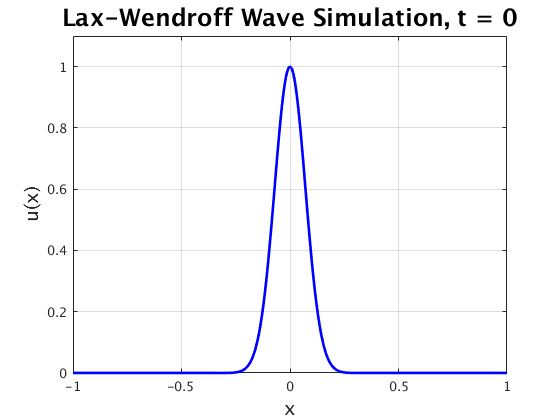
\includegraphics[width=0.75\textwidth]{wave_0}
    \caption{Initial state of the system.}
    \label{fig:wave0}
\end{figure}

\begin{figure}[H]
    \centering
    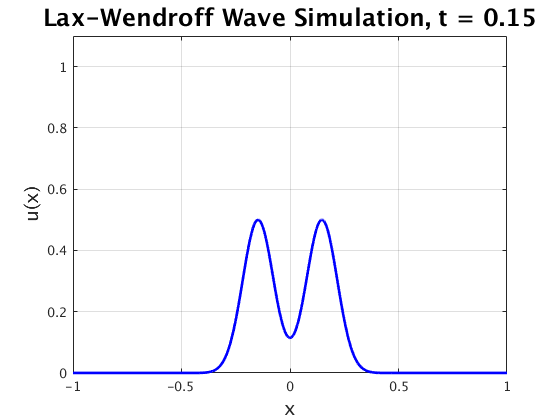
\includegraphics[width=0.75\textwidth]{wave_1}
    \caption{The initial condition beginning to split.}
    \label{fig:wave1}
\end{figure}

\begin{figure}[H]
    \centering
    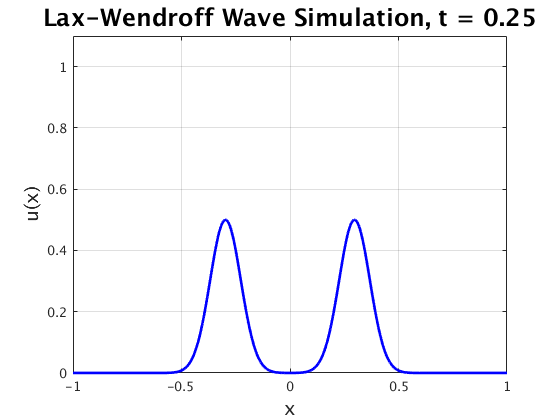
\includegraphics[width=0.75\textwidth]{wave_2}
    \caption{Full split, waves propagating away from origin.}
    \label{fig:wave2}
\end{figure}
\end{document}
